\documentclass{zkdl-template}

\usepackage{opencolor}

\title{\huge\sffamily\bfseries ZKDL Camp Lecture Notes}
\author{\Large\sffamily Distributed Lab}
%\date{\sffamily \today}
%\titlepic{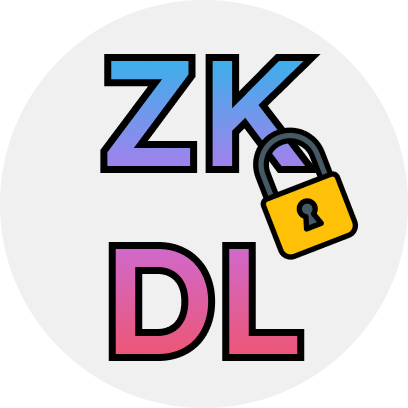
\includegraphics[width=0.2\textwidth]{lectures/images/common/logo.png}}

\begin{document}

\pagestyle{fancy}

% --- Drawing a book cover ---

\colorlet{coverBackground}{oc-gray-0}
\colorlet{coverBoxBackground}{oc-gray-7}

\pagecolor{coverBackground}
\begin{tcolorbox}[
    standard jigsaw,
    colframe=coverBoxBackground, 
    colback=oc-gray-3,
    width=\textwidth, 
    halign=center, 
    valign=center, 
    %opacityback=0,
    arc=1em,
    shadow={4mm}{-3mm}{0mm}{black!30!white},
    enhanced,
    boxrule=5pt,
    rightrule=9pt,
    bottomrule=9pt]
    \maketitle
\end{tcolorbox}

% Include figure below

\vspace{1.5cm}
\begin{figure}[h]
    \centering
    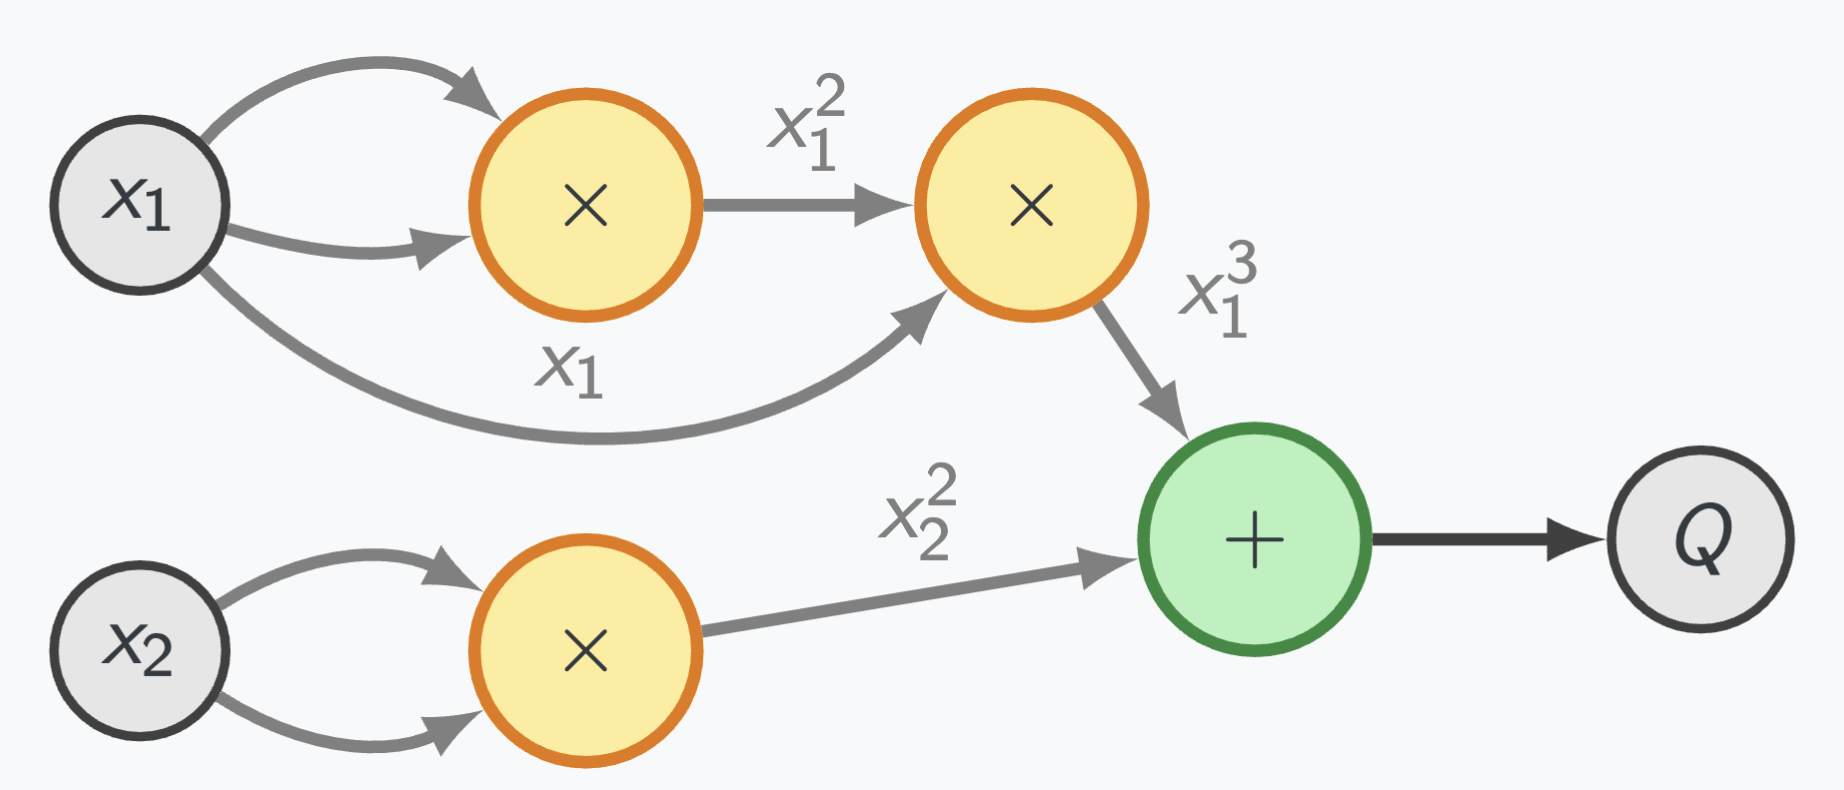
\includegraphics[width=0.8\textwidth]{lectures/images/cover-image-1.png}
\end{figure}

\pagebreak

% --- Table of Contents ---

\pagecolor{white}

\tableofcontents

\pagebreak

% --- Content ---

\section{Group Theory and Polynomials}

\subfile{lectures/1-math}

\section{Basics of Security Analysis}\label{section:math-crypto-2}

\subfile{lectures/2-math-and-crypto}

\section{Field Extensions and Elliptic Curves}

\subfile{lectures/3-ec}

\section{Projective Coordinates and Pairing}

\subfile{lectures/4-pairing}

\section{Commitment Schemes}

\subfile{lectures/5-commitments}

\section{Introduction to Zero-Knowledge Proofs}

\subfile{lectures/6-intro-zk}

\section{Sigma Protocols}

\subfile{lectures/7-sigma}

\section{Introduction to SNARKs. Arithmetic Circuits. R1CS}

\subfile{lectures/8-circuits}

\section{Quadratic Arithmetic Program. Probabilistically Checkable Proofs}

\subfile{lectures/9-qap-pcp}

\section{Pairing-based SNARKs. Pinocchio and Groth16}

\subfile{lectures/10-groth}

\end{document}
